%% bare_conf.tex
%% V1.4b
%% 2015/08/26
%% by Michael Shell
%% See:
%% http://www.michaelshell.org/
%% for current contact information.
%%
%% This is a skeleton file demonstrating the use of IEEEtran.cls
%% (requires IEEEtran.cls version 1.8b or later) with an IEEE
%% conference paper.
%%
%% Support sites:
%% http://www.michaelshell.org/tex/ieeetran/
%% http://www.ctan.org/pkg/ieeetran
%% and
%% http://www.ieee.org/

%%*************************************************************************
%% Legal Notice:
%% This code is offered as-is without any warranty either expressed or
%% implied; without even the implied warranty of MERCHANTABILITY or
%% FITNESS FOR A PARTICULAR PURPOSE! 
%% User assumes all risk.
%% In no event shall the IEEE or any contributor to this code be liable for
%% any damages or losses, including, but not limited to, incidental,
%% consequential, or any other damages, resulting from the use or misuse
%% of any information contained here.
%%
%% All comments are the opinions of their respective authors and are not
%% necessarily endorsed by the IEEE.
%%
%% This work is distributed under the LaTeX Project Public License (LPPL)
%% ( http://www.latex-project.org/ ) version 1.3, and may be freely used,
%% distributed and modified. A copy of the LPPL, version 1.3, is included
%% in the base LaTeX documentation of all distributions of LaTeX released
%% 2003/12/01 or later.
%% Retain all contribution notices and credits.
%% ** Modified files should be clearly indicated as such, including  **
%% ** renaming them and changing author support contact information. **
%%*************************************************************************


% *** Authors should verify (and, if needed, correct) their LaTeX system  ***
% *** with the testflow diagnostic prior to trusting their LaTeX platform ***
% *** with production work. The IEEE's font choices and paper sizes can   ***
% *** trigger bugs that do not appear when using other class files.       ***                          ***
% The testflow support page is at:
% http://www.michaelshell.org/tex/testflow/



\documentclass[conference,10pt]{IEEEtran}
% Some Computer Society conferences also require the compsoc mode option,
% but others use the standard conference format.
%
% If IEEEtran.cls has not been installed into the LaTeX system files,
% manually specify the path to it like:
% \documentclass[conference]{../sty/IEEEtran}

\usepackage[utf8]{inputenc}



% Some very useful LaTeX packages include:
% (uncomment the ones you want to load)


% *** MISC UTILITY PACKAGES ***
%
%\usepackage{ifpdf}
% Heiko Oberdiek's ifpdf.sty is very useful if you need conditional
% compilation based on whether the output is pdf or dvi.
% usage:
% \ifpdf
%   % pdf code
% \else
%   % dvi code
% \fi
% The latest version of ifpdf.sty can be obtained from:
% http://www.ctan.org/pkg/ifpdf
% Also, note that IEEEtran.cls V1.7 and later provides a builtin
% \ifCLASSINFOpdf conditional that works the same way.
% When switching from latex to pdflatex and vice-versa, the compiler may
% have to be run twice to clear warning/error messages.






% *** CITATION PACKAGES ***
%
%\usepackage{cite}
% cite.sty was written by Donald Arseneau
% V1.6 and later of IEEEtran pre-defines the format of the cite.sty package
% \cite{} output to follow that of the IEEE. Loading the cite package will
% result in citation numbers being automatically sorted and properly
% "compressed/ranged". e.g., [1], [9], [2], [7], [5], [6] without using
% cite.sty will become [1], [2], [5]--[7], [9] using cite.sty. cite.sty's
% \cite will automatically add leading space, if needed. Use cite.sty's
% noadjust option (cite.sty V3.8 and later) if you want to turn this off
% such as if a citation ever needs to be enclosed in parenthesis.
% cite.sty is already installed on most LaTeX systems. Be sure and use
% version 5.0 (2009-03-20) and later if using hyperref.sty.
% The latest version can be obtained at:
% http://www.ctan.org/pkg/cite
% The documentation is contained in the cite.sty file itself.






% *** GRAPHICS RELATED PACKAGES ***
%
\ifCLASSINFOpdf
  \usepackage[pdftex]{graphicx}
  % declare the path(s) where your graphic files are
  \graphicspath{{./images/}{./plots/}}
  % and their extensions so you won't have to specify these with
  % every instance of \includegraphics
  \DeclareGraphicsExtensions{.pdf,.jpeg,.png}
\else
  % or other class option (dvipsone, dvipdf, if not using dvips). graphicx
  % will default to the driver specified in the system graphics.cfg if no
  % driver is specified.
  % \usepackage[dvips]{graphicx}
  % declare the path(s) where your graphic files are
  % \graphicspath{{../eps/}}
  % and their extensions so you won't have to specify these with
  % every instance of \includegraphics
  % \DeclareGraphicsExtensions{.eps}
\fi
% graphicx was written by David Carlisle and Sebastian Rahtz. It is
% required if you want graphics, photos, etc. graphicx.sty is already
% installed on most LaTeX systems. The latest version and documentation
% can be obtained at: 
% http://www.ctan.org/pkg/graphicx
% Another good source of documentation is "Using Imported Graphics in
% LaTeX2e" by Keith Reckdahl which can be found at:
% http://www.ctan.org/pkg/epslatex
%
% latex, and pdflatex in dvi mode, support graphics in encapsulated
% postscript (.eps) format. pdflatex in pdf mode supports graphics
% in .pdf, .jpeg, .png and .mps (metapost) formats. Users should ensure
% that all non-photo figures use a vector format (.eps, .pdf, .mps) and
% not a bitmapped formats (.jpeg, .png). The IEEE frowns on bitmapped formats
% which can result in "jaggedy"/blurry rendering of lines and letters as
% well as large increases in file sizes.
%
% You can find documentation about the pdfTeX application at:
% http://www.tug.org/applications/pdftex





% *** MATH PACKAGES ***
%
\usepackage{amsmath}
% A popular package from the American Mathematical Society that provides
% many useful and powerful commands for dealing with mathematics.
%
% Note that the amsmath package sets \interdisplaylinepenalty to 10000
% thus preventing page breaks from occurring within multiline equations. Use:
\interdisplaylinepenalty=2500
% after loading amsmath to restore such page breaks as IEEEtran.cls normally
% does. amsmath.sty is already installed on most LaTeX systems. The latest
% version and documentation can be obtained at:
% http://www.ctan.org/pkg/amsmath





% *** SPECIALIZED LIST PACKAGES ***
%
\usepackage{algorithmic}
% algorithmic.sty was written by Peter Williams and Rogerio Brito.
% This package provides an algorithmic environment fo describing algorithms.
% You can use the algorithmic environment in-text or within a figure
% environment to provide for a floating algorithm. Do NOT use the algorithm
% floating environment provided by algorithm.sty (by the same authors) or
% algorithm2e.sty (by Christophe Fiorio) as the IEEE does not use dedicated
% algorithm float types and packages that provide these will not provide
% correct IEEE style captions. The latest version and documentation of
% algorithmic.sty can be obtained at:
% http://www.ctan.org/pkg/algorithms
% Also of interest may be the (relatively newer and more customizable)
% algorithmicx.sty package by Szasz Janos:
% http://www.ctan.org/pkg/algorithmicx




% *** ALIGNMENT PACKAGES ***
%
%\usepackage{array}
% Frank Mittelbach's and David Carlisle's array.sty patches and improves
% the standard LaTeX2e array and tabular environments to provide better
% appearance and additional user controls. As the default LaTeX2e table
% generation code is lacking to the point of almost being broken with
% respect to the quality of the end results, all users are strongly
% advised to use an enhanced (at the very least that provided by array.sty)
% set of table tools. array.sty is already installed on most systems. The
% latest version and documentation can be obtained at:
% http://www.ctan.org/pkg/array


% IEEEtran contains the IEEEeqnarray family of commands that can be used to
% generate multiline equations as well as matrices, tables, etc., of high
% quality.




% *** SUBFIGURE PACKAGES ***
%\ifCLASSOPTIONcompsoc
%  \usepackage[caption=false,font=normalsize,labelfont=sf,textfont=sf]{subfig}
%\else
% \usepackage[caption=false,font=footnotesize]{subfig}
%\fi
% subfig.sty, written by Steven Douglas Cochran, is the modern replacement
% for subfigure.sty, the latter of which is no longer maintained and is
% incompatible with some LaTeX packages including fixltx2e. However,
% subfig.sty requires and automatically loads Axel Sommerfeldt's caption.sty
% which will override IEEEtran.cls' handling of captions and this will result
% in non-IEEE style figure/table captions. To prevent this problem, be sure
% and invoke subfig.sty's "caption=false" package option (available since
% subfig.sty version 1.3, 2005/06/28) as this is will preserve IEEEtran.cls
% handling of captions.
% Note that the Computer Society format requires a larger sans serif font
% than the serif footnote size font used in traditional IEEE formatting
% and thus the need to invoke different subfig.sty package options depending
% on whether compsoc mode has been enabled.
%
% The latest version and documentation of subfig.sty can be obtained at:
% http://www.ctan.org/pkg/subfig




% *** FLOAT PACKAGES ***
%
%\usepackage{fixltx2e}
% fixltx2e, the successor to the earlier fix2col.sty, was written by
% Frank Mittelbach and David Carlisle. This package corrects a few problems
% in the LaTeX2e kernel, the most notable of which is that in current
% LaTeX2e releases, the ordering of single and double column floats is not
% guaranteed to be preserved. Thus, an unpatched LaTeX2e can allow a
% single column figure to be placed prior to an earlier double column
% figure.
% Be aware that LaTeX2e kernels dated 2015 and later have fixltx2e.sty's
% corrections already built into the system in which case a warning will
% be issued if an attempt is made to load fixltx2e.sty as it is no longer
% needed.
% The latest version and documentation can be found at:
% http://www.ctan.org/pkg/fixltx2e


%\usepackage{stfloats}
% stfloats.sty was written by Sigitas Tolusis. This package gives LaTeX2e
% the ability to do double column floats at the bottom of the page as well
% as the top. (e.g., "\begin{figure*}[!b]" is not normally possible in
% LaTeX2e). It also provides a command:
%\fnbelowfloat
% to enable the placement of footnotes below bottom floats (the standard
% LaTeX2e kernel puts them above bottom floats). This is an invasive package
% which rewrites many portions of the LaTeX2e float routines. It may not work
% with other packages that modify the LaTeX2e float routines. The latest
% version and documentation can be obtained at:
% http://www.ctan.org/pkg/stfloats
% Do not use the stfloats baselinefloat ability as the IEEE does not allow
% \baselineskip to stretch. Authors submitting work to the IEEE should note
% that the IEEE rarely uses double column equations and that authors should try
% to avoid such use. Do not be tempted to use the cuted.sty or midfloat.sty
% packages (also by Sigitas Tolusis) as the IEEE does not format its papers in
% such ways.
% Do not attempt to use stfloats with fixltx2e as they are incompatible.
% Instead, use Morten Hogholm'a dblfloatfix which combines the features
% of both fixltx2e and stfloats:
%
% \usepackage{dblfloatfix}
% The latest version can be found at:
% http://www.ctan.org/pkg/dblfloatfix




% *** PDF, URL AND HYPERLINK PACKAGES ***
%
\usepackage{url}
% url.sty was written by Donald Arseneau. It provides better support for
% handling and breaking URLs. url.sty is already installed on most LaTeX
% systems. The latest version and documentation can be obtained at:
% http://www.ctan.org/pkg/url
% Basically, \url{my_url_here}.




% *** Do not adjust lengths that control margins, column widths, etc. ***
% *** Do not use packages that alter fonts (such as pslatex).         ***
% There should be no need to do such things with IEEEtran.cls V1.6 and later.
% (Unless specifically asked to do so by the journal or conference you plan
% to submit to, of course. )


% correct bad hyphenation here
\hyphenation{op-tical net-works semi-conduc-tor}

% other packages\
\usepackage[inline]{enumitem}
% \usepackage{listings}
\usepackage{minted}
\usepackage{todonotes}
\usepackage{caption}
\usepackage{subcaption}
\usepackage{xcolor}
\usepackage[detect-weight=true,detect-family=true,binary-units=true,list-units=single,range-units=single]{siunitx}
\usepackage[nolist]{acronym}
\begin{acronym}
  \acro{CPS}{Cyber-Physical System}
  \acro{NCS}{Networked Control System}
  \acroindefinite{NCS}{an}{a}
  \acro{LAN}{Local-Area Network}
  \acro{WLAN}{Wireless Local-Area Network}
  \acro{KPI}{Key Performance Indicator}
  \acro{WPAN}{Wireless Personal Area Network}
  \acro{CSMA/CD}{Carrier-Sense Multiple Acess with Collision Detection}
  \acro{CLEAVE}{ControL bEnchmArking serVice on the Edge}
  \acro{OS}{Operating System}
  \acro{UDP}{User Datagram Protocol}
  \acro{TCP}{Transmission Control Protocol}
  \acro{RMS}{Root Mean Square}
  \acro{RTT}{Round-Trip Time}
  \acro{CI}{Confidence Interval}
  \acro{AP}{Access Point}
\end{acronym}
\usepackage{booktabs}
% \usepackage{graphicx}

% references
\usepackage[
  style=ieee,
  sorting=none,
  sortcites,
  hyperref,
  mincitenames=1,
  maxcitenames=2,
  maxbibnames=2,
  minbibnames=1,
  citestyle=numeric-comp, % for [1, 2] instead of [1], [2]
  backend=biber
]{biblatex}
\bibliography{bibliography.bib}
\usepackage{orcidlink}

\usepackage{hyperref}
\usepackage[noabbrev,nameinlink]{cleveref}
\crefname{subfigure}{subfigure}{subfigures} \Crefname{subfigure}{Subfigure}{Subfigures}

% links
\hypersetup{
    colorlinks,
    linkcolor={red!80!black},
    citecolor={blue!80!black},
    urlcolor={blue!80!black}
}

\AtBeginBibliography{\small}
\newcommand{\email}[1]{\href{mailto:#1}{\texttt{#1}}}
\begin{document}

\title{CLEAVE Paper for CNERT'22}


% author names and affiliations
% use a multiple column layout for up to three different
% affiliations
\author{
  \IEEEauthorblockN{Manuel {Olguín Muñoz}\IEEEauthorrefmark{1}~\orcidlink{0000-0002-3383-2335}, James Gross\IEEEauthorrefmark{2}~\orcidlink{0000-0001-6682-6559}}
  \IEEEauthorblockA{
    School of Electrical Engineering\\and Computer Science\\
    KTH Royal Institute of Technology\\
    Stockholm, Sweden\\
    \IEEEauthorrefmark{1}\email{molguin@kth.se}, \IEEEauthorrefmark{2}\email{jamesgr@kth.se}
  }
  % \and
  % \IEEEauthorblockN{James Gross~\orcidlink{0000-0001-6682-6559}}
  % \IEEEauthorblockA{
  %   School of Electrical Engineering\\and Computer Science\\
  %   KTH Royal Institute of Technology\\
  %   Stockholm, Sweden\\
  %   \email{jamesgr@kth.se}
  % }
}

% conference papers do not typically use \thanks and this command
% is locked out in conference mode. If really needed, such as for
% the acknowledgment of grants, issue a \IEEEoverridecommandlockouts
% after \documentclass

% for over three affiliations, or if they all won't fit within the width
% of the page, use this alternative format:
% 
%\author{\IEEEauthorblockN{Michael Shell\IEEEauthorrefmark{1},
%Homer Simpson\IEEEauthorrefmark{2},
%James Kirk\IEEEauthorrefmark{3}, 
%Montgomery Scott\IEEEauthorrefmark{3} and
%Eldon Tyrell\IEEEauthorrefmark{4}}
%\IEEEauthorblockA{\IEEEauthorrefmark{1}School of Electrical and Computer Engineering\\
%Georgia Institute of Technology,
%Atlanta, Georgia 30332--0250\\ Email: see http://www.michaelshell.org/contact.html}
%\IEEEauthorblockA{\IEEEauthorrefmark{2}Twentieth Century Fox, Springfield, USA\\
%Email: homer@thesimpsons.com}
%\IEEEauthorblockA{\IEEEauthorrefmark{3}Starfleet Academy, San Francisco, California 96678-2391\\
%Telephone: (800) 555--1212, Fax: (888) 555--1212}
%\IEEEauthorblockA{\IEEEauthorrefmark{4}Tyrell Inc., 123 Replicant Street, Los Angeles, California 90210--4321}}




% use for special paper notices
%\IEEEspecialpapernotice{(Invited Paper)}




% make the title area
\maketitle

\begin{abstract}
    In this work, we present \acs*{CLEAVE}, a novel, completely software based framework for repeatable and scalable experimentation in \acfp*{NCS}.
    While these systems have long been a subject of both theoretical and experimental research, their inter-domain nature  has led to a wide number of task-specific approaches to research, and little work has been devoted to generalizable, repeatable, and scalable experimentation.
    We aim to tackle this gap in knowledge through an approach based on the emulation of physical plants which communicate over a real network with controllers implemented in software.
    \acs*{CLEAVE} is furthermore designed and built for the edge, using Python3 and with full compatibility with industry-standard containerization solutions.
    Although designed for single-loop emulations, the flexibility afforded by the aformentioned characteristics allow our framework to be adaptated to and employed in a multitude of more complex scenarios.

    We validate \acs*{CLEAVE} using an initial implementation of an inverted pendulum \acs*{NCS}.
    Our results showcase the utility of the tool as a repeatable, extensible, and scalable solution to \acs*{NCS} performance evaluation and benchmarking.
\end{abstract}

% no keywords

% For peer review papers, you can put extra information on the cover
% page as needed:
% \ifCLASSOPTIONpeerreview
% \begin{center} \bfseries EDICS Category: 3-BBND \end{center}
% \fi
%
% For peerreview papers, this IEEEtran command inserts a page break and
% creates the second title. It will be ignored for other modes.
% \IEEEpeerreviewmaketitle

% actual paper

\section{Introduction}\label{sec:intro}

The number and applications of \acp{CPS}~\cite{Rajkumar2010CPS} --- that is, systems in which a real, physical mechanism is controlled by a computer --- have exploded in later years.
This rise in popularity is in great part driven by the advent of novel wireless communication technologies as well as networking paradigms, such as cellular 5G and Edge Computing.

In particular, \acp{NCS}~\cite{Gupta2010NCSOverview}, a type of \ac{CPS} wherein multiple networked actuators and sensors form a part of the same automatic control system, have been of great interest to the scientific community in the last decade.
Due to their potential advantages for industrial settings~\cite{Lu2015WSAN}, a large body of work exists dedicated to the modelling and performance characterization of these systems~\cite{Hespanha2007Survey,Zhang2013Survey,Zhang2016Survey}.
\Acp{NCS} enhance the flexibility of and improve existing control systems by allowing for the distribution of control functions over and across networks.
This allows for --- for instance --- simultaneous centralized coordination, control, and monitoring of potentially hundreds of devices.

Most of the large literature concerning \acp{NCS}, however, follows a theoretical approach, and only a small fraction of it deals with experimental studies.
The inherent inter-domain nature of \acp{NCS}, which intertwines knowledge from the fields of communications, computing, and control theory, coupled with the complexity of experimental platforms make these kinds of studies hard to perform.

The most straightforward approach to experimental research in \ac{NCS} use setups in which the complete system uses real hardware.
\textcite{Drew2005NCSWLAN} present \iac{NCS} model which considers both random packet delay and loss on both the sensor and actuator sides of the feedback loop; \textcite{Baumann2018LowPower}, on the other hand, develop an evaluation methodology for wireless \ac{NCS}.
Both works validate their results on physical testbeds, consisting of inverted penduli plants controlled wirelessly over IEEE 802.11 WiFi from a central computation point.
Similarly, \textcite{Li2014Wireless} implement a wireless microcontroller-based system for vibration control and validate it on a physical prototype consisting of a cantilever beam controlled over an IEEE 802.15.4 \ac{WPAN} system.
\textcite{Cuenca2019UAV} design and implement periodic event-triggered sampling and dual-rate control techniques for wireless control, validating their contributions on a four-rotor autonomous drone platform controlled over WiFi.

Conversely, some studies choose to instead use completely \emph{simulated} \ac{NCS} setups~\cite{Andersson2005Simulation,Eyisi2012NCSWT}.
Such an approach is employed by \textcite{Du2009Smith}; the authors develop a novel \emph{Smith} predictor to compensate for varying latencies in wireless \acp{NCS} and validate it using the \emph{TrueTime}~\cite{Henriksson2002TrueTime} simulator.
In \textcite{Chen2015synccontrol} the authors validate and evaluate a number of synchronous control strategies for three-motor setups using completely simulated \acp{NCS} environments.
\citeauthor{Wu2012NPC} introduce the concept of \emph{network predictive control} in\ \cite{Wu2012NPC} and use it to balance a simulated inverted pendulum over a simulated wireless network.
In \cite{Ma2019DynamicSched}, \citeauthor{Ma2019DynamicSched} propose an optimal dynamic scheduling strategy that optimizes performance of multi-loop control systems and validate it by simulating a four-loop control system over an IEEE 802.15.4 \ac{WPAN}.


Finally, a number of experimental studies instead employ \emph{hardware-} and \emph{network-in-the-loop} approaches.
Hardware-in-the-loop refers to \ac{NCS} setups in which a real network interacts with a simulated or emulated control system.
This kind of setup is particularly prevalent in the field of \emph{smart grid} control, and has been used by studies such as \textcite{Wang2020VoltageControl}, in which the authors validate a novel three-level coordinated control method for photovoltaic inverters.

On the other hand, network-in-the-loop refers to experimental setups in which the \emph{network} is instead simulated or emulated.
An example of this approach can be found in \textcite{Natale2004InvPendEthernet}, in which the authors interface an real inverted pendulum system with an emulated IEEE 802.3 Ethernet network to study the effects of the \ac{CSMA/CD} medium access control scheme on plant stability.

As evidence by the discussion above, experimental research in \acp{NCS} includes a large variety of heterogeneous hardware and software platforms, as well as methodologies and \acp{KPI}.
This, in turn, leads to hardware, software, and methodology fragmentation, as different studies tend to prefer approaches more favored in their respective communities.
Furthermore, existing studies tend to focus on individual aspects and components of a system, thus producing results which do not provide a complete image of the \ac{NCS}.
We identify thus a gap in knowledge pertaining to the reproducibility and comparison of experimental studies on these systems.

\textcite{Zoppi2020NCSBench} made a first attempt at tackling this challenge with their \emph{NCSbench} platform.
\emph{NCSbench} is an open-source \ac{NCS} benchmarking platform designed with reproducibility in mind, built using the \citetitle{LEGOMindstormsEV3}~\cite{LEGOMindstormsEV3} platform.
It allows for easy and highly reproducible experimentation and benchmarking of \acp{NCS}, due to its low-cost, accessibility, and ease of reconfiguration.

Although the work of \textcite{Zoppi2020NCSBench} is a relevant and important step towards the reproducibility of \ac{NCS} benchmarks, we believe it still falls short on some aspects.
In particular, we argue the reliance of \emph{NCSbench} on specific hardware --- accessible as it may be --- hampers the potential of the platform, as it fundamentally limits both the physical systems that can be benchmarked and the scalability of the performed benchmarks.

In this paper, we present thus the first fully-software-based \ac{NCS} benchmarking framework with scalability and repeatability as its main focus.
This framework is built on top of the \emph{Python 3.8}~\cite{Python3.8} language, making it highly extensible and able to harness the tremendous amount of already existing user-provided libraries and packages~\cite{pypi}.
Additionally, it is fully compatible with \emph{containerization} technologies such as \emph{Docker}~\cite{merkel2014docker}, making it suitable for automated deployment and benchmarking on industry-standard deployment using container orchestration technologies.
We name this framework \ac{CLEAVE}.

The rest of this paper is structured as follows.
\Cref{sec:approach} presents the design principles of the framework.
Next, in \cref{sec:experiments}, we present a series of experiments which validate the utility, flexibility, and repeatability of \ac{CLEAVE}.
Finally, we conclude this paper in \cref{sec:conclusion} with a brief discussion on the strengths and weaknesses of the platform, as well as on future directions to take.
\section{The \ac{CLEAVE} framework}\label{sec:approach}

In this section, we present and detail our \ac{CLEAVE} framework for the performance evaluation of \aclp{NCS}, with a particular focus on edge deployments.
Our design follows a virtualized emulation approach; we provide a framework for the real-time \emph{emulation} of physical control systems and the easy implementation of softwarized controllers which interact with \emph{real} networks.
In other words, \ac{CLEAVE} is a platform with an easy-to-use \ac{API} on which a multitude of \ac{NCS} types can be emulated.
This allows for great flexibility, as the core components of the \ac{NCS} can easily be switched out while maintaining the realism of the network, arguably the most complex and limiting component of edge \acp{NCS}.

The framework is distributed as \emph{free and open-source} softwarethrough the \emph{GitHub} organization of the \emph{KTH ExPECA} research group\footnote{\url{https://github.com/KTH-EXPECA/CLEAVE}}.
Furthermore, we plan to eventually provide an open library of \ac{NCS} implementations, thus making the tool even more accessible to the community.

\subsection{Design and Implementation}

\cref{fig:cleave:ncs:struct} shows an overview of the conceptual structure and operation of \ac{CLEAVE}.
The \emph{State} implements the discrete-time behavior of the Plant.
At the beginning of each time-step, actuated variables in the \emph{State} are updated with values obtained from the \emph{Actuator} objects.
Conversely, at the end of each time-step, sensed variables are sampled and used to update values associated with \emph{Sensor} objects.
These values are processed at the \emph{Sensors} (e.g.\ to add noise) before being sent over the network to the \emph{Controller}.
The \emph{Controller} calculates actuation values and updates the \emph{Actuators} over the network.
Finally, the \emph{Actuators} process the actuation values and hold the results until they are read at the next time-step.

Implementation-wise, \ac{CLEAVE} is built on top of the well-established and stable \emph{Twisted}\footnote{\url{https://twistedmatrix.com}} asynchronous programming and networking framework.
The aforementioned core components (\emph{State}, \emph{Controller}, \emph{Sensors}, and \emph{Actuators}) are provided as \acp{ABC} with core functionality that users must extend for their specific use cases and \acp{NCS}.
The framework makes no assumptions about the inner workings of the user implementations of these classes other than the interfaces they expose.
Users are therefore free to implement arbitrarily complex functionality in these components.
On the other hand, \ac{CLEAVE} handles network communication and metric collection autonomously; users only need to select the desired transport protocol (we do however provide an \ac{API} for extending the available transports).

Below we present a brief overview of the design and implementation of the core components.

\begin{description}[style=nextline]
    \item[State Base Class]
    
    \ac{ABC} with an abstract method
    \mintinline{python}{advance()} which users must extend with the implementation of discrete-time emulation of the plant side of the \ac{NCS}.
    The \mintinline{python}{advance()} method is called by the framework periodically according to the configured emulation update rate, and should perform a single time-step of the discrete-time emulation.
    Two additional, optionally extensible methods, \mintinline{python}{initialize()} and \mintinline{python}{shutdown()}, are provided for users to implement single-fire set-up and tear-down procedures.

    % This class also provides functionality for the automatic tracking and updating of sensed and actuated values.
    % This is handled through special auxiliary classes, \emph{SensorVariable} and \emph{ActuatorVariable}, which when instantiated and assigned to an attribute of the \emph{State} allow the framework to track and modify them.

    \item[Controller Base Class]
    
    Defines a single abstract method \mintinline{python}{process()}, which takes a mapping of names to values corresponding to the sensed variables of the \emph{State}, and must return a similar mapping corresponding to the actuated variables.
    This method is called by \ac{CLEAVE} in an event-based manner whenever samples are received from the plant side; however, we intend to extend this implementation to time-interval-based approaches eventually as well.

    \item[Sensor Base Class]
    
    \emph{Sensors} implement the processing of monitored stated variables before sending them over the network to the \emph{Controller}.
    This base class must be initialized with a property name (corresponding to the monitored \emph{State} attribute) and a sampling rate in \si{\hertz}, and provides an abstract method \mintinline{python}{process_sample()} which must be extended with an implementation of the processing performed on each sample.

    \item[Actuator Base Class] 
    
    Finally, \emph{Actuators} perform the processing of actuation values obtained over the network from the \emph{Controller}.
    The base class is initialized with a property name corresponding to the name of the actuated \emph{State} attribute, and provides two abstract methods which must be implemented by extending classes:
    \begin{enumerate*}[itemjoin={{; }}, itemjoin*={{; and }}]
        \item \mintinline{python}{set_value()}, which is called by the framework whenever a new value for the corresponding actuated attribute is received
        \item \mintinline{python}{get_actuation()}, which is called on every time-step and must return a value to apply to the actuated attribute.
    \end{enumerate*}

\end{description}


\subsection{Configuring and Executing \iac{NCS}}

Once the core components for the emulation have been defined and implemented, they need to be registered with the framework.
This is done through Python scripts which simply define a number of required (and some optional) top-level variables, corresponding to emulation parameters such as the \emph{State}, \emph{Controller}, \emph{Sensor}, and \emph{Actuator} subclasses to use; the emulation update rate; the controller-side host and address; data output directories; \emph{et cetera}.
These Python configuration files are then provided as arguments to the \texttt{cleave} command line provided by the framework.
\ac{CLEAVE} imports and parses them, and then sets up and executes the emulation.

Although the core design of \ac{CLEAVE} follows a single-loop approach, multi-loop scenarios can be easily implemented through the combination of multiple \ac{CLEAVE} instances.
Furthermore, the framework makes no assumptions about the individual components other than the signatures of methods on the base classes that must be extended and implemented.
Combined with the plain-Python emulation configuration scripts, this makes development of more complex scenarios merely a matter of implementing the desired functionality within the framework itself.

\subsection{Current Implementations}

\begin{figure}
    \centering
    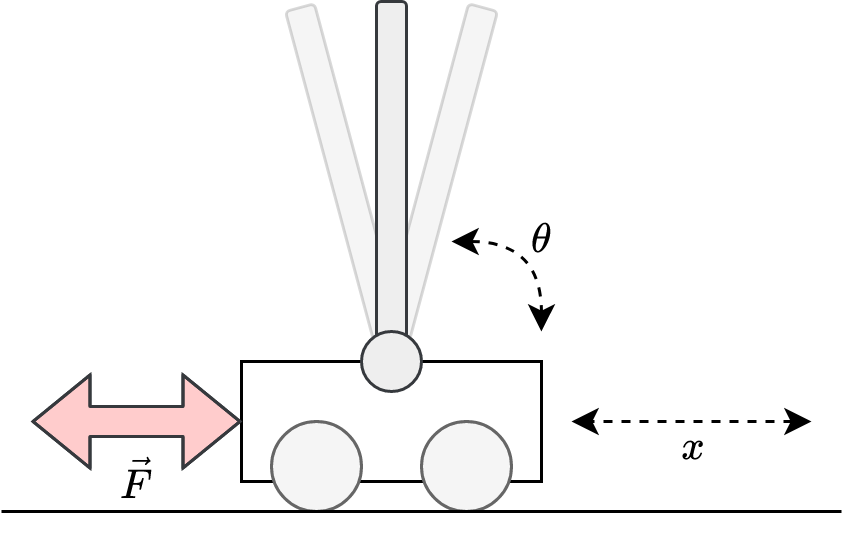
\includegraphics[width=.7\columnwidth]{images/inverted_pendulum.png}
    \caption{
        The 2d inverted pendulum system.
    }\label{fig:invpend}
\end{figure}

For the purpose of this work, we have used \ac{CLEAVE} to implement an emulated \emph{inverted pendulum} control loop (see \cref{fig:invpend}), the goal of which is to balance the vertically free-swinging pendulum by applying horizontal forces on the cart.
We have chosen this system as an initial benchmark for its relative simplicity as well as prevalence in the field of automatic control as one of the fundamental examples of linear control.
However, as mentioned above, we eventually plan to build an open library of emulated control loops.  

The inverted pendulum plant \emph{State} is implemented as a real-time discrete-time physical emulation using CLEAVE's API and a 2D physics library\footnote{Pymunk: \url{http://www.pymunk.org/en/latest/}}, updated at a constant \SI{120}{\hertz} (this value is configurable; in this case it corresponds to the maximum achievable stable rate on the clients).
\emph{Sensors} for the angle, position, angular velocity, and velocity of the \emph{State}, and an \emph{Actuator} for the horizontal force applied to the cart are implemented as ``perfect'', i.e.\ values are returned as-is, without any added noise.
For the controller side, a proportional-differential strategy is implemented using the framework \emph{Controller} API and the \emph{NumPy} numeric computation library\footnote{NumPy: \url{https://numpy.org/}}.
Plant and controller are then packaged into containers, for ease of orchestration and reparametrization, and to mimic real-world deployment.

\section{Experimental validation}\label{sec:experiments}

In this section, we demonstrate the utility of \ac{CLEAVE} through a series of experiments on an emulated \ac{NCS} running on a number of client devices and a cloudlet.
We aim to answer questions relating to the ability of our framework to provide accurate and repeatable measurements of the performance of \acp{NCS} deployed on edge computing infrastructure.

This section is structured in two parts.
\Cref{ssec:expsetup} details the experimental setup and describes the experiments performed.
\Cref{ssec:results} then presents and discusses the numerical results.

\subsection{Experimental Setup}\label{ssec:expsetup}

We detail our experimental edge setup in \cref{fig:cleave:expsetup,tab:hardware}.
It consists of \num{10} Raspberry Pi 4B  clients connected wirelessly to an IEEE 802.11n \ac{AP}; connected to the Ethernet backbone of this \ac{AP} is a general-purpose Cloudlet.
On top of this physical architecture we configure a Docker Swarm\footnote{Swarm mode overview: \url{https://docs.docker.com/engine/swarm/}} managed centrally from the Cloudlet.
For each experimental scenario we deploy a number of control loops inside this Swarm, executing plant containers exclusively in the Raspberry Pi clients (up to a single plant per client) and controller containers in the Cloudlet.
Plants and controllers communicate using the \ac{UDP} over an overlay network which sits on top of and abstracts away the real network configuration.
Additionally, to obtain baseline results without the stochastic effects of the network, we employ a secondary ``local-only'' setup, in which plants and controllers are executed co-located on the Cloudlet.

% Please add the following required packages to your document preamble:
% \usepackage{booktabs}
% \usepackage{graphicx}
\begin{table}[]
    \centering
    \caption{Hardware used in the experiments.}\label{tab:hardware}
    \resizebox{\columnwidth}{!}{%
    \begin{tabular}{@{}llrrrl@{}}
    \toprule
    \multicolumn{1}{c}{\textbf{}} &
      \multicolumn{1}{c}{\textbf{CPU}} &
      \multicolumn{1}{c}{\textbf{\begin{tabular}[c]{@{}c@{}}Freq\\ {[}\si{\giga\hertz}{]}\end{tabular}}} &
      \multicolumn{1}{c}{\textbf{\begin{tabular}[c]{@{}c@{}}Core\\ Count\end{tabular}}} &
      \multicolumn{1}{c}{\textbf{\begin{tabular}[c]{@{}c@{}}RAM\\ {[}\si{\giga\byte}{]}\end{tabular}}} &
      \multicolumn{1}{c}{\textbf{\begin{tabular}[c]{@{}c@{}}Operating\\ System\end{tabular}}} \\ \midrule
    \textbf{Cloudlet} &
      \begin{tabular}[c]{@{}l@{}}Intel\textregistered{} Core\texttrademark{}\\ i7-8700\end{tabular} &
      \num{3.2} &
      \num{6} &
      \num{32} &
      \begin{tabular}[c]{@{}l@{}}Ubuntu Server \\20.04 LTS \\Kernel v5.4.0\\\ \end{tabular} \\
    \textbf{Client} &
      \begin{tabular}[c]{@{}l@{}}Cortex-A72\\ (ARM v8)\end{tabular} &
      \num{2.0} &
      \num{4} &
      \num{8} &
      \begin{tabular}[c]{@{}l@{}}Ubuntu Server \\20.04 LTS \\Kernel v5.4.0\end{tabular} \\ \bottomrule
    \end{tabular}%
    }
\end{table}

\begin{figure}
    \centering
    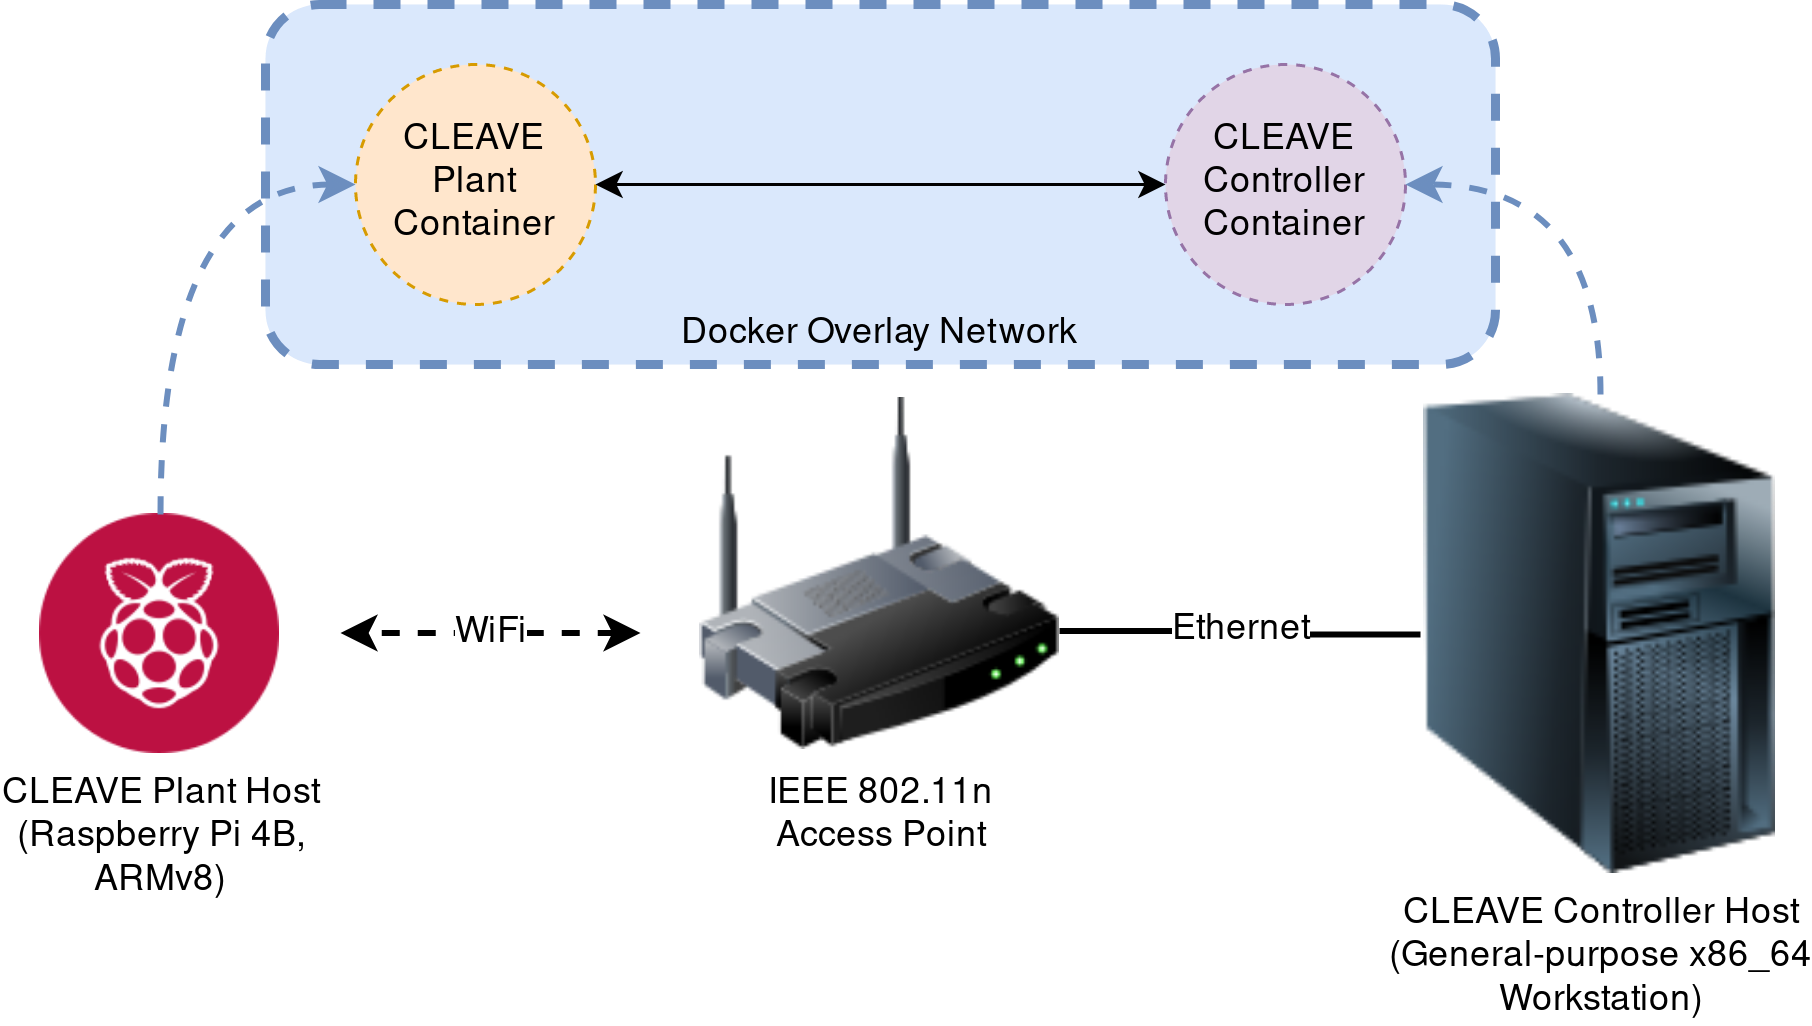
\includegraphics[width=.95\columnwidth]{images/CLEAVE_experiment_setup}
    \caption{
        The setup used for our experimentation. 
        % Containerized versions of the core CLEAVE emulation components are deployed inside a Docker Swarm Overlay Network spanning \num{10} Raspberry Pi 4B clients connected to a single Cloudlet over an IEEE 802.11n \ac{AP}.
    }\label{fig:cleave:expsetup}
\end{figure}

\begin{figure*}[h]
    \centering
    \begin{subfigure}[t]{.5\textwidth}
        \centering
        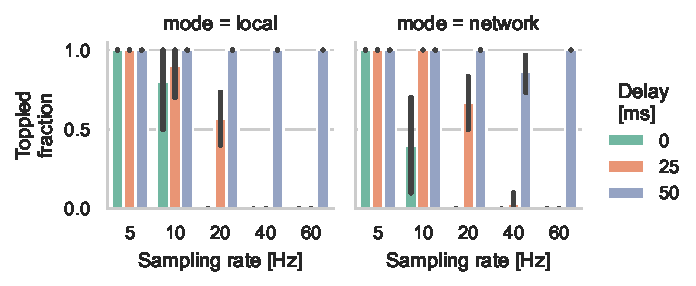
\includegraphics[width=.9\textwidth]{single_loop_toppled}
        % \todo[inline]{Check consistency??}
        \caption{}%
        \label{fig:single:topple}
    \end{subfigure}%
    \begin{subfigure}[t]{.5\textwidth}
        \centering
        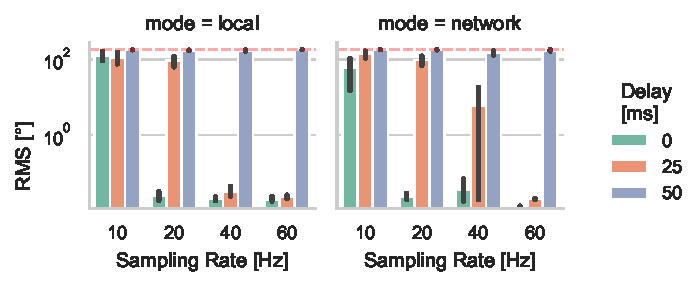
\includegraphics[width=.9\textwidth]{single_loop_rms}
        % \todo[inline]{Mark fully toppled experiments with an X.}
        \caption{}\label{fig:single:rms}
    \end{subfigure}%
    \caption[caption]{
        Stability metrics for the single-loop scenarios.
        \labelcref{fig:single:topple} shows the fraction of plants that toppled, per experimental setup.
        \labelcref{fig:single:rms} shows the mean \ac{RMS} value of the angle with respect to the vertical axis in logarithmic scale; the red line indicates \( y = 180 \).
        Error bars indicate \SI{95}{\percent} \acp{CI} in both plots.
        }%
    \label{fig:single:stability}
\end{figure*}

\begin{figure}
    \centering
    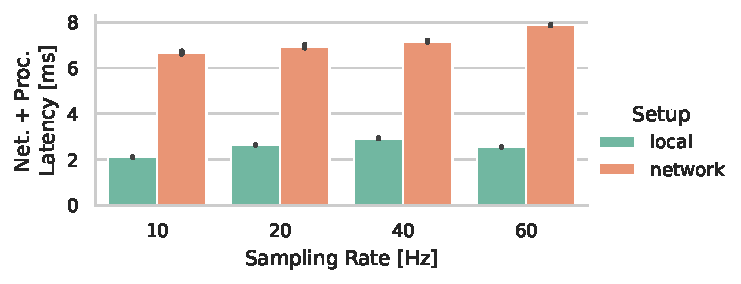
\includegraphics[width=.9\columnwidth]{single_loop_rtts}
    \caption{
        Mean latency due to network and processing for both single-loop scenarios.
        Error bars indicate \SI{95}{\percent} \acp{CI}.
    }\label{fig:single:rtt}
\end{figure}

\begin{figure*}[t]
    \centering
    \begin{subfigure}[h]{.25\textwidth}
        \centering
        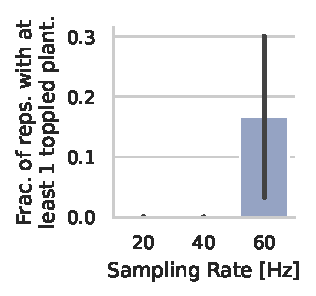
\includegraphics[width=.9\textwidth]{video_topple_frac}
        \caption{}\label{fig:video:toppled}
    \end{subfigure}%
    \begin{subfigure}[h]{.25\textwidth}
        \centering
        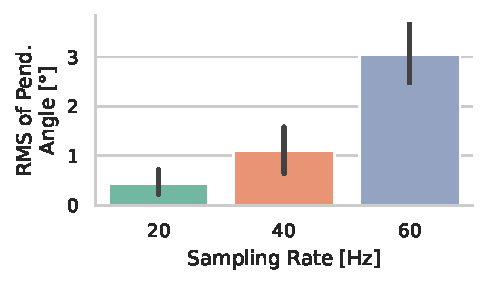
\includegraphics[width=.9\textwidth]{video_angle_rms}
        \caption{}\label{fig:video:rms}
    \end{subfigure}%
    \begin{subfigure}[h]{.25\textwidth}
        \centering
        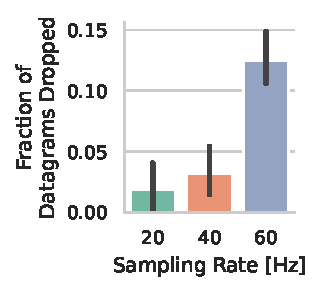
\includegraphics[width=.9\textwidth]{video_drop_frac}
        \caption{}\label{fig:video:drop}
    \end{subfigure}%
    \begin{subfigure}[h]{.25\textwidth}
        \centering
        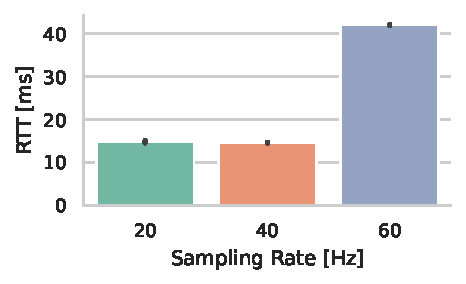
\includegraphics[width=.9\textwidth]{video_rtt}
        \caption{}\label{fig:video:rtt}
    \end{subfigure}%
    \caption{
        Results for the realistic scenario.
        \labelcref{fig:video:toppled} shows the fraction of repetitions of each scenario in which \emph{at least} one plant failed to maintain stability and toppled.
        \labelcref{fig:video:rms} shows the \ac{RMS} for the pendulum angles for each scenario, only considering data from plants that did not topple.
        \labelcref{fig:video:drop} shows the fraction of \ac{UDP} datagrams dropped, averaged over all plants and repetitions per scenario.
        \labelcref{fig:video:rtt} shows the measured end-to-end plant-side \ac{RTT}, averaged over all plants and repetitions per scenario.
        Error bars indicate \SI{95}{\percent} \ac{CI} in all plots.
    }\label{fig:video:results}
\end{figure*}

\subsubsection{Single Loop Baseline Scenarios}

We first run a series of single loop scenarios with varying parametrization of the \ac{NCS}, intended as initial baselines to evaluate the accuracy of the \ac{CLEAVE} framework and showcase its flexibility.

For these scenarios, we vary:
\begin{enumerate*}[itemjoin={{; }}, itemjoin*={{; and }}]
    \item the sampling rate of the Plant state, setting it to \SIlist[list-final-separator={, or }]{10;20;40;60}{\hertz}
    \item the responsiveness of the Controller, adding fixed delays of \SIlist[list-final-separator={, or }]{0;25;50}{\milli\second} after the processing of each sample.
\end{enumerate*}

We repeat each combination of these parameters at least \num{10} times, for both the networked and ``local-only'' setups; experiments with sampling rates \( \geq \) \SI{20}{\hertz} and artificial delays \( \geq \) \SI{25}{\milli\second} were repeated an additional \num{20} times for better statistical significance.
Each repetition lasts for \SI{5}{\minute}, during which we collect detailed data on both the state of the controlled system as well as on the data sent over the network.

Scenarios are executed automatically in batches using a simple Python script which interacts with Docker through the widely adopted \emph{docker-py}\footnote{Docker SDK for Python: \url{https://docker-py.readthedocs.io/en/stable/}} library.
This is \ac{CLEAVE}'s first advantage over existing frameworks; it is designed with cloud and edge technology and paradigms in mind, making integration with existing systems straightforward.

\subsubsection{Realistic Scenario with Network Resource Contention}

Next, we run a multi-loop scenario to validate the utility of \ac{CLEAVE} in a more realistic setting where network resources are shared with video stream traffic.
Video analytics is one of the main proposed use cases for edge computing~\cite{Ananthanarayanan2017Analytics,Yi2017Analytics,Wang2018Analytics}, and thus we foresee edge \ac{NCS} deployments being deployed in parallel with such applications in the future.

In this scenario, we deploy \num{6} control loops on the experimental setup depicted in \cref{fig:cleave:expsetup}.
On the remaining \num{4} clients we run the \emph{iperf3}\footnote{iperf3: \url{https://iperf.fr/}} traffic load generator, each generating \SI[per-mode=symbol]{6.5}{\mega\bit\per\second} of uplink \ac{UDP} traffic.
This emulates the load generated on the network by \SI{1080}{p} Full-HD video streaming, originating from the clients and terminating in the cloudlet.
We execute this scenario with \ac{NCS} plant sampling rates of \SIlist{20;40;60}{\hertz}.
Each sampling rate configuration is run for \SI{5}{\minute}, and then repeated \num{30} times to obtain statistical significance.
Once again, repetitions of this scenario are executed automatically in batches using a simple Python script and \emph{docker-py}.

\subsection{Results}\label{ssec:results}

The results presented below provide valuable insights on both system limits and on the chosen \ac{NCS} itself, as well as on the capabilities of \ac{CLEAVE}.

\subsubsection{Single Plant Scenario}

We begin with a simple analysis of the stability of the Plant, as \ac{CLEAVE} allows for straightforward and repeatable collection and posterior processing of relevant metrics.  
\cref{fig:single:stability} shows the results relating to the stability of the plants in the single-loop scenarios:
\cref{fig:single:topple} shows the fraction of plants that toppled in each scenario, and \cref{fig:single:rms} shows the average \ac{RMS} for the absolute pendula angles.
Toppled plants were identified simply by analysis of the emulation data; instances whose pendulum angles reached values above a threshold\footnote{This value depends on the parametrization of the controller; in this case it corresponds to \SI{0.35}{\radian}.} were marked as ``toppled''.

As expected, higher sampling rates tend to correlate with better quality of control; at higher sampling rates the system was able to reach stability at higher \acp{RTT}.
These initial results already hint at interesting consequences for \ac{NCS} deployments on the edge.
For instance, it is clear from \cref{fig:single:stability} that network delays can, to a certain extent, be compensated for by increasing the sampling rate of the system.
A corollary of this is, conversely, that at lower network latencies \acp{NCS} are able to stabilize at lower sampling rates.
Adaptive sampling might thus be a viable method for optimizing \ac{NCS} resource utilization at the edge.

For completeness, we also showcase \ac{CLEAVE}'s ability to obtain network performance data from the experiments.
\cref{fig:single:rtt} shows average latency due to network and processing (excluding synthetic delays) for both single-loop scenarios.
Packet losses were below \SI{0.2}{\percent} for all parametrizations of the single-loop scenario over the network, and \SI{0}{\percent} for all parametrizations of the local-only setup.

\subsubsection{Realistic Scenario}

\cref{fig:video:results} shows a summary of the results obtained from the realistic scenario.
These results are interesting in their counter-intuitiveness.
Conventional wisdom would lead us to think that higher sampling rates are always better for the stability of control systems; however, \cref{fig:video:toppled,fig:video:rms} clearly show this not to be the case for \ac{NCS} in resource-constrained scenarios.
\SI{60}{\hertz} was the least stable configuration, with at least one pendulum toppling in around \SI{16}{\percent} of the repetitions, and mean pendulum angle \ac{RMS} circa \num{3} times that of the \SI{40}{\hertz} scenario.
\SI{40}{\hertz} was in turn the second worst configuration --- although it presented no toppled pendula, average angle \ac{RMS} doubled that of the \SI{20}{\hertz} setup.

We can see an explanation for these behaviors in \cref{fig:video:drop,fig:video:rtt}.
Whereas both the \SIlist{20;40}{\hertz} setups show losses well below \SI{5}{\percent}, the \SI{60}{\hertz} scenario shows an average of around \SI{13}{\percent} of datagrams lost.
The differences in \acp{RTT} results are equally telling; \acp{RTT} for the \SI{60}{\hertz} scenario were on average approx.\ \num{3} times those for the \SIlist{20;40}{\hertz} setups.

%(circa \SI{41}{\milli\second} versus \SIrange[range-phrase=--]{13}{15}{\milli\second}).

These results stem from the contention for network resources, and hint at important trade-offs system designers will have to take into consideration when designing and developing \acp{NCS} for deployment on the edge.
The edge will be \emph{multi-tenant} and \emph{multi-instance}. 
\ac{NCS} deployments will have to be designed with shared resources in mind, and given the complexity of these systems, experimental tools like \ac{CLEAVE} will be key for their succesful adoption and massification.

\section{Conclusion}\label{sec:conclusion}

The issue of repeatable and scalable benchmarks has been largely glossed over in \ac{NCS} literature, as existing experimental research studies tend to implement \emph{ad-hoc} solutions.

In this work, we aim to tackle this issue by presenting a fully software-based framework for repeatable, reproducible, and easily scalable \ac{NCS} benchmarking with a particular focus on edge deployment.
Our framework, \ac{CLEAVE}, allows for the easy implementation of emulated \acp{NCS} on real networks.
It is fully parametrizable, extendable, and built with industry-standard edge technologies and paradigms in mind.
We validate the utility of this tool through a series of scenarios; our results showcase the ability of the framework to extract relevant metrics relating to the stability of the control system, as well as on the performance of the underlying network link.
We believe \ac{CLEAVE} represents an important step towards enabling inexpensive and low-complexity scalable research for real-world deployment of edge-bound \acp{NCS}.

There is still, however, work to be done.
We are extending the number of plant and controller implementations on the framework, with the goal of creating an open library of \acp{NCS} to share with the community.
At the moment, the interactions of \ac{CLEAVE} and tools such as Docker are still quite superficial.
Our goal is to achieve a much tighter integration, e.g.\ by providing the toolkit as pre-packaged container images.
Finally, the validity of the results obtained by the framework will have to be verified through more thorough, realistic scenarios than what we have been able to show in this work.
In particular, we intend to perform large-scale experimentation targetting 5G cellular deployments, as this technology is set to become the backbone of edge networks in the near future.

\section*{Acknowledgements}\label{sec:acks}

This research has been partially funded by
\begin{enumerate*}[itemjoin={{; }}, itemjoin*={{; and }}]
    \item the VINNOVA Competence Center for \ac{TECoSA} at KTH Royal Institute of Technology
    \item the \ac{SSF}, through grant number ITM17--0246, awarded to James Gross, Ph.D.
\end{enumerate*}
Any opinions, findings, conclusions or recommendations expressed in this material are those of the authors and do not necessarily reflect the view(s) of their employers or funding sources.

We also wish to thank S. Mostafavi, V. N. Moothedath, M. Alsakati, O. Ferm, S. Vojcic, and A. Bhattacharya for their effort and support for this work.


% trigger a \newpage just before the given reference
% number - used to balance the columns on the last page
% adjust value as needed - may need to be readjusted if
% the document is modified later
%\IEEEtriggeratref{8}
% The "triggered" command can be changed if desired:
%\IEEEtriggercmd{\enlargethispage{-5in}}

% references section

% can use a bibliography generated by BibTeX as a .bbl file
% BibTeX documentation can be easily obtained at:
% http://mirror.ctan.org/biblio/bibtex/contrib/doc/
% The IEEEtran BibTeX style support page is at:
% http://www.michaelshell.org/tex/ieeetran/bibtex/
%\bibliographystyle{IEEEtran}
% argument is your BibTeX string definitions and bibliography database(s)
%\bibliography{IEEEabrv,../bib/paper}
%
% <OR> manually copy in the resultant .bbl file
% set second argument of \begin to the number of references
% (used to reserve space for the reference number labels box)

% \nocite{*}
\printbibliography{}
% that's all folks
\end{document}


